\subsubsection{Ý tưởng}
\textbf{Shell Sort} là một cải tiến của thuật toán \textbf{Insertion Sort}. Ý tưởng chính là sắp xếp các phần tử nằm xa nhau trước, sau đó giảm dần khoảng cách giữa các phần tử so sánh, và cuối cùng thực hiện một lần \textbf{Insertion Sort} với các khoảng cách bằng 1. Điều này giúp giảm số lần hoán đổi và so sánh khi so sánh các phần tử gần nhau ở bước cuối.

\subsubsection{Mã giả}
\begin{algorithm}[H]
\caption{ShellSort}
\begin{algorithmic}[1]
\Procedure{\textbf{ShellSort}}{$arr, n$}
    \State \textbf{Input:} Mảng $arr$ gồm $n$ phần tử
    \State \textbf{Output:} Mảng $arr$ được sắp xếp
    \State $gap \gets n/2$
    \While {$gap > 0$}
        \For {$i \gets gap$ \textbf{to} $n - 1$} 
            \State $temp \gets arr[i]$
            \State $j \gets i$
            \While{$j \geq gap$ \textbf{and} $arr[j - gap] > temp$}
                \State $arr[j] \gets arr[j - gap]$
                \State $j \gets j - gap$
            \EndWhile
            \State $arr[j] \gets temp$
        \EndFor
        \State $gap \gets gap / 2$
    \EndWhile
\EndProcedure
\end{algorithmic}
\end{algorithm}
\subsubsection{Ví dụ}
Dưới đây là các bước chạy tay của thuật toán \textbf{Shell Sort}:
\begin{figure}[H]
    \centering
    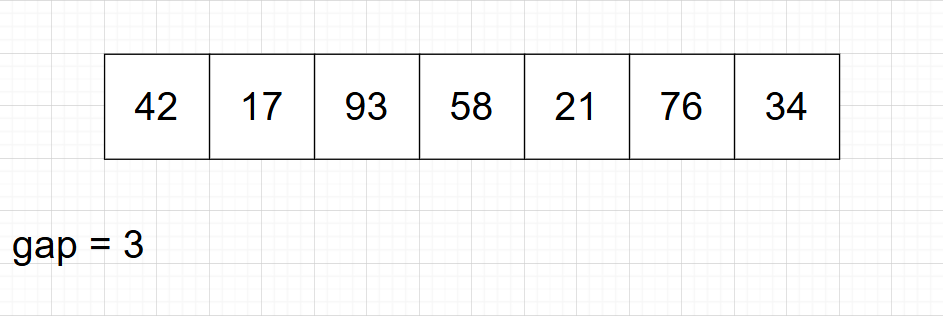
\includegraphics[width=1\linewidth]{img/shell_sort/1.png}
    \vspace{0.15cm}
    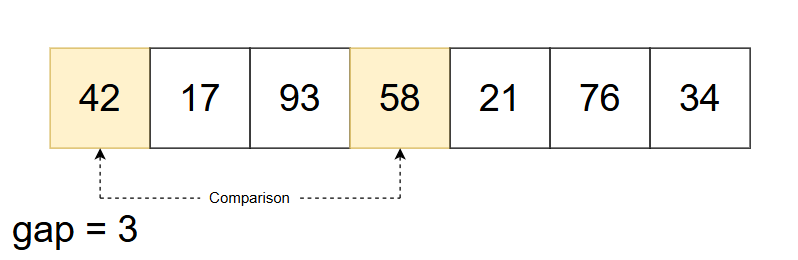
\includegraphics[width=1\linewidth]{img/shell_sort/2.png}
    \vspace{0.15cm}
    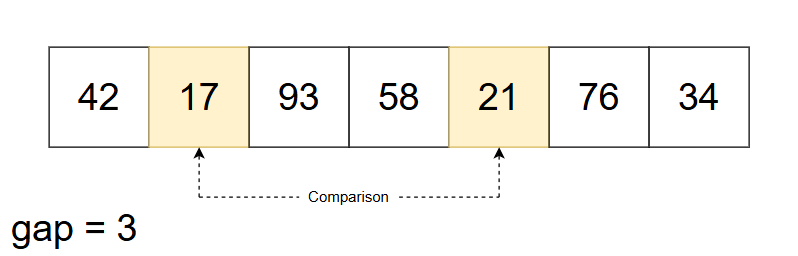
\includegraphics[width=1\linewidth]{img/shell_sort/3.png}
    \vspace{0.15cm}
    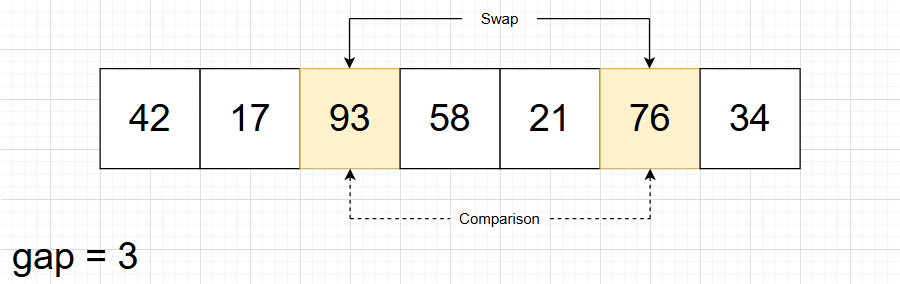
\includegraphics[width=1\linewidth]{img/shell_sort/4.png}
    \caption{Các bước chạy - 1}
    \label{fig:part1}
\end{figure}

\begin{figure}[H]
    \centering
    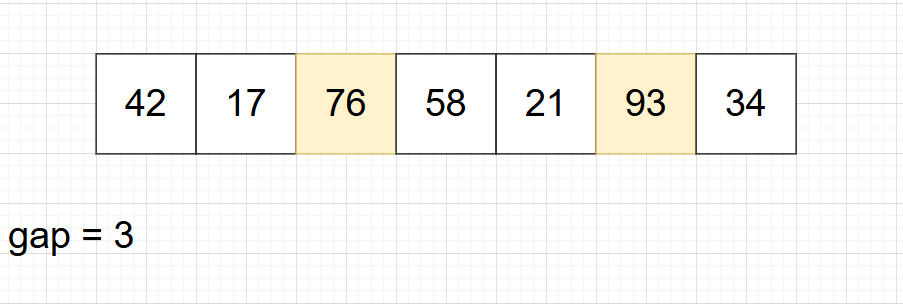
\includegraphics[width=1\linewidth]{img/shell_sort/5.png}
    \vspace{0.5cm}
    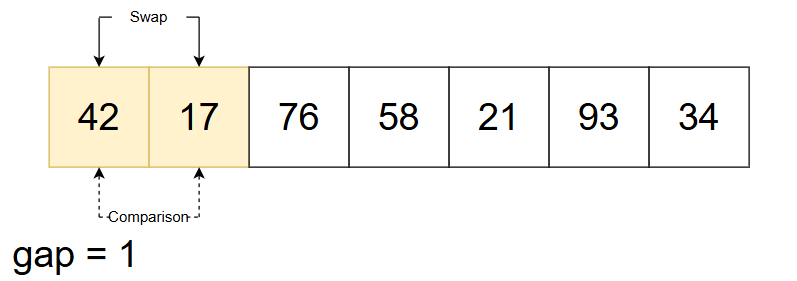
\includegraphics[width=1\linewidth]{img/shell_sort/6.png}
    \vspace{0.15cm}
    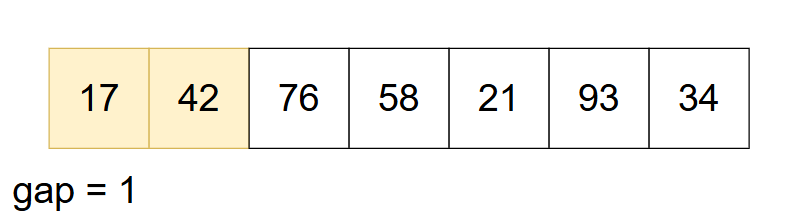
\includegraphics[width=1\linewidth]{img/shell_sort/7.png}
    \vspace{0.15cm}
    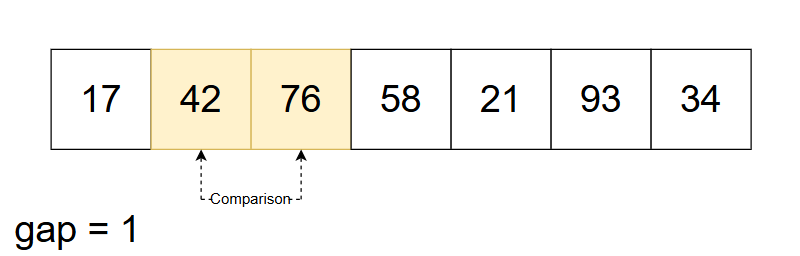
\includegraphics[width=1\linewidth]{img/shell_sort/8.png}
    \caption{Các bước chạy - 2}
    \label{fig:part2}
\end{figure}

\begin{figure}[H]
    \centering
    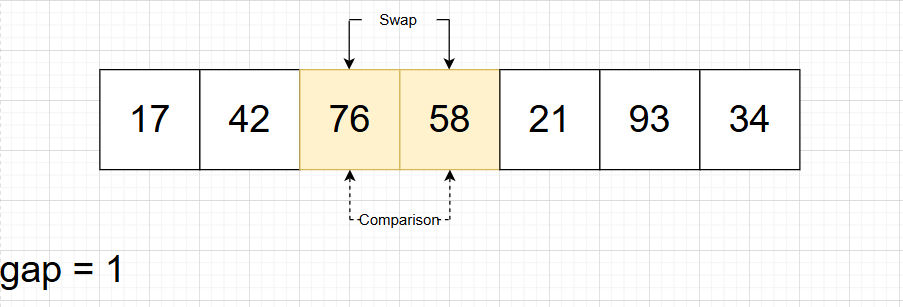
\includegraphics[width=1\linewidth]{img/shell_sort/09.png}
    \vspace{0.15cm}
    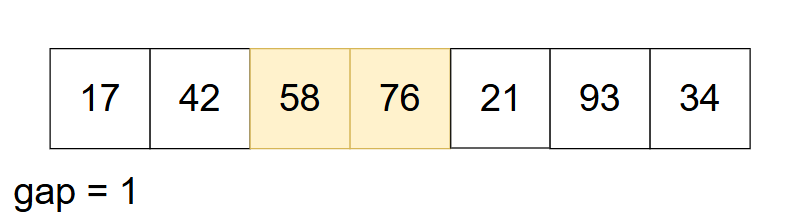
\includegraphics[width=1\linewidth]{img/shell_sort/10.png}
    \vspace{0.15cm}
    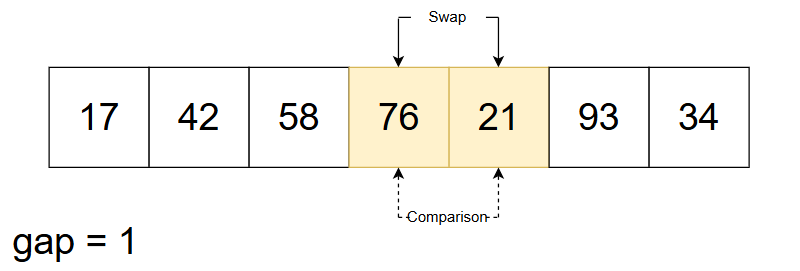
\includegraphics[width=1\linewidth]{img/shell_sort/11.png}
    \vspace{0.15cm}
    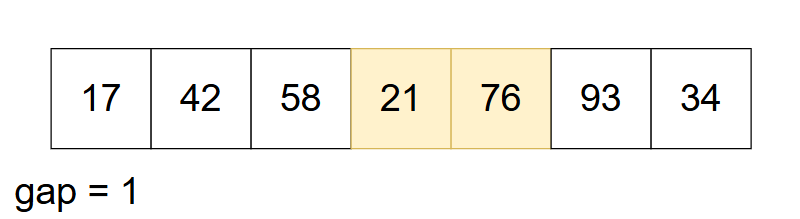
\includegraphics[width=1\linewidth]{img/shell_sort/12.png}
    \caption{Các bước chạy - 3}
    \label{fig:part3}
\end{figure}

\begin{figure}[H]
    \centering
    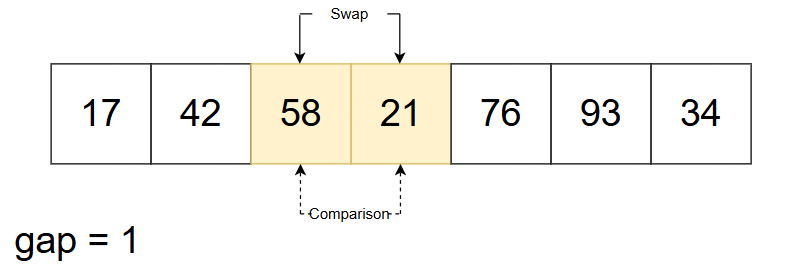
\includegraphics[width=1\linewidth]{img/shell_sort/13.png}
    \vspace{0.15cm}
    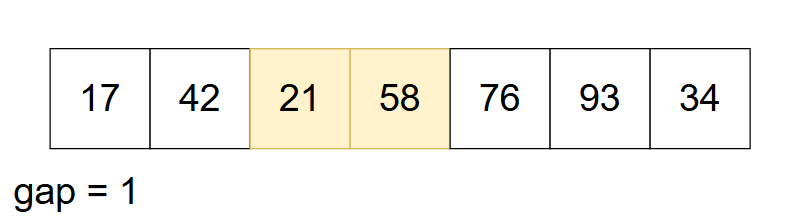
\includegraphics[width=1\linewidth]{img/shell_sort/14.png}
    \vspace{0.15cm}
    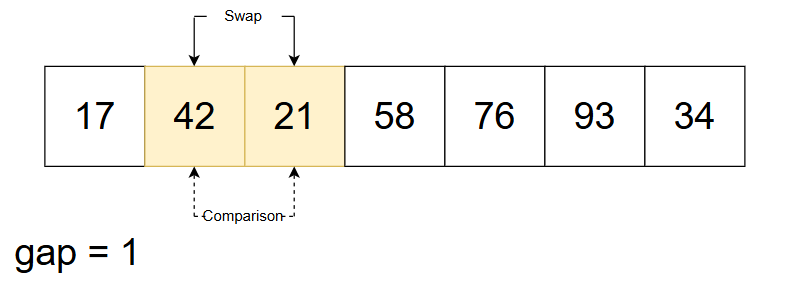
\includegraphics[width=1\linewidth]{img/shell_sort/15.png}
    \vspace{0.15cm}
    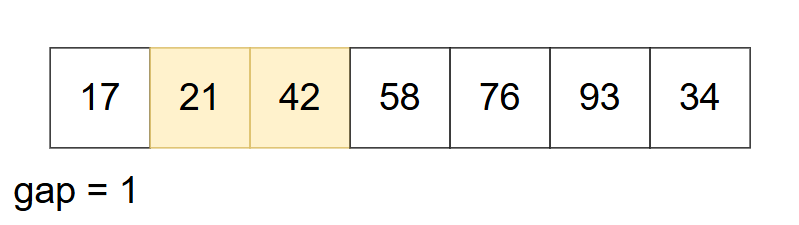
\includegraphics[width=1\linewidth]{img/shell_sort/16.png}
    \caption{Các bước chạy - 4}
    \label{fig:part4}
\end{figure}

\begin{figure}[H]
    \centering
    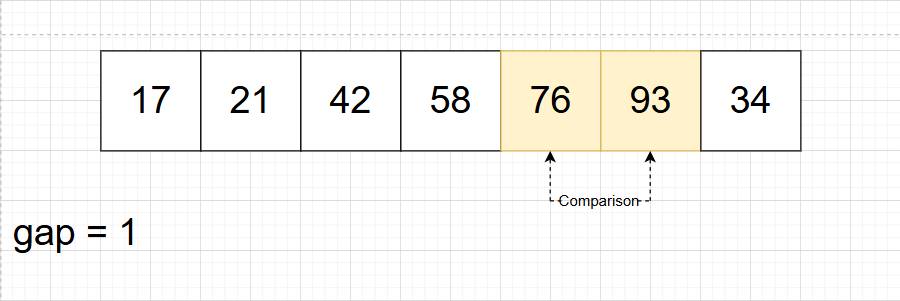
\includegraphics[width=1\linewidth]{img/shell_sort/17.png}
    \vspace{0.15cm}
    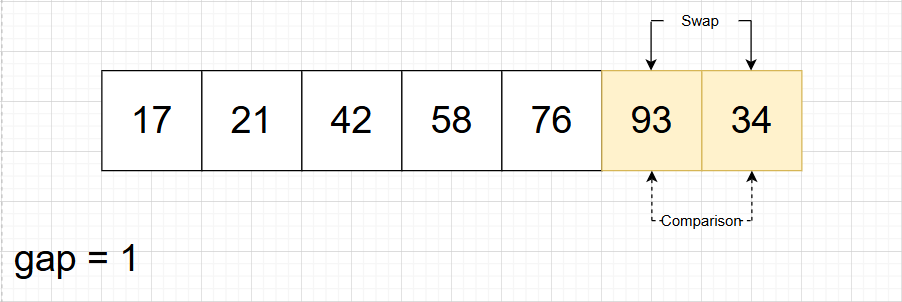
\includegraphics[width=1\linewidth]{img/shell_sort/18.png}
    \vspace{0.15cm}
    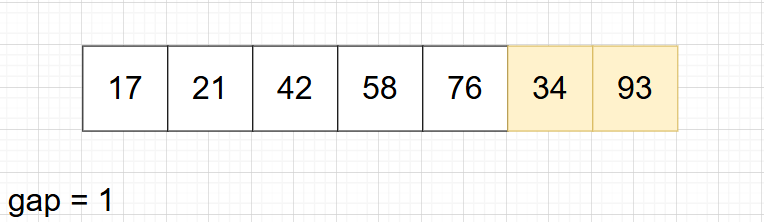
\includegraphics[width=1\linewidth]{img/shell_sort/19.png}
    \vspace{0.15cm}
    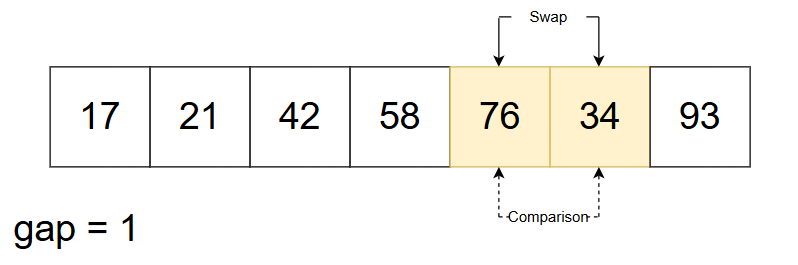
\includegraphics[width=1\linewidth]{img/shell_sort/20.png}
    \caption{Các bước chạy - 5}
    \label{fig:part5}
\end{figure}

\begin{figure}[H]
    \centering
    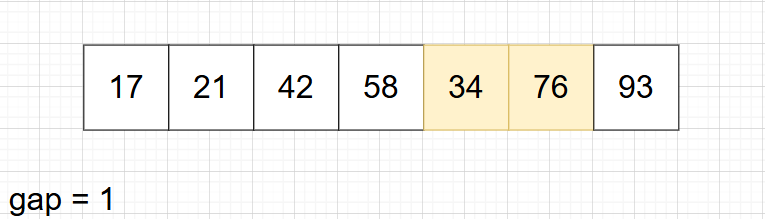
\includegraphics[width=1\linewidth]{img/shell_sort/21.png}
    \vspace{0.15mm}
    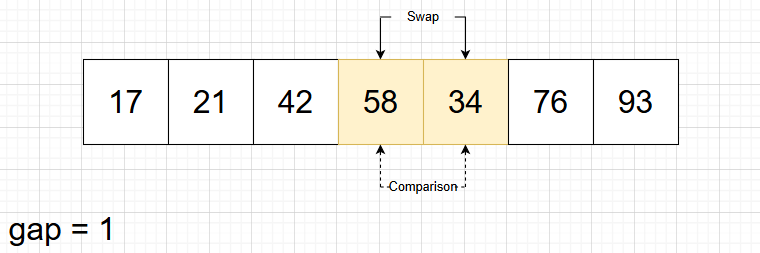
\includegraphics[width=1\linewidth]{img/shell_sort/22.png}
    \vspace{0.15mm}
    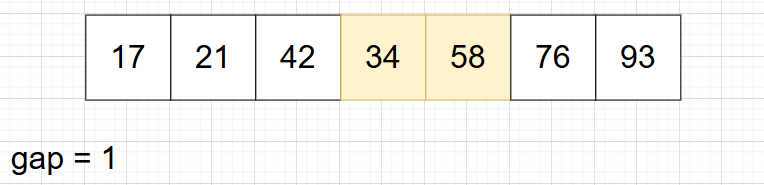
\includegraphics[width=1\linewidth]{img/shell_sort/23.png}
    \vspace{0.15mm}
    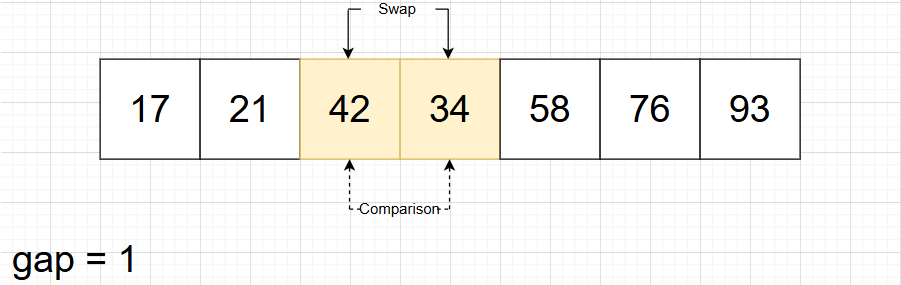
\includegraphics[width=1\linewidth]{img/shell_sort/24.png}
    \vspace{0.15mm}
    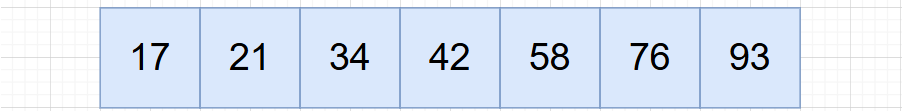
\includegraphics[width=1\linewidth]{img/shell_sort/25.png}
    \caption{Các bước chạy - 6}
    \label{fig:part6}
\end{figure}

\subsubsection{Độ phức tạp}
\begin{itemize}
    \item[\textbf{--}]Độ phức tạp về thời gian:
        \begin{itemize}
<<<<<<< HEAD
            \item[$\bullet$] \textbf{Best Case:} $\mathcal{O}(n \cdot \log{}n)$
            \item[$\bullet$] \textbf{Average Case:}  $\mathcal{O}(n^2)$
            \item[$\bullet$] \textbf{Worst Case:}  $\mathcal{O}(n^2)$
        \end{itemize}
    \item[\textbf{--}]Độ phức tạp về không gian: $\mathcal{O}(n)$ 
=======
            \item[$\bullet$] \textbf{Best Case:} $O(n \cdot \log{n})$ (phụ thuộc vào cách chọn $gap$)
            \item[$\bullet$] \textbf{Average Case:}  $O(n^{3/2})$ (với chuỗi $gap$ \textbf{Knuth} hoặc \textbf{Hibbard})
            \item[$\bullet$] \textbf{Worst Case:}  $O(n^2)$ (với chuỗi $gap$ đơn giản như chia đôi liên tiếp)
        \end{itemize}
    \item[\textbf{--}]Độ phức tạp về không gian: $O(1)$ 
>>>>>>> 425c4b7 (hoàn chỉnh thuật shellsort)
    \item[\textbf{--}]Tính ổn định: Không ổn định
\end{itemize}